\section{InsightCAD}

\subsection{Introduction}

InsightCAD is a script-based tool for creating three-dimensional geometry models. 
All geometric operations are based on the OpenCASCADE geometry kernel. 
It uses the boundary representation approach (BREP) for treating the geometry. Thus it is possible to import and export the common exchange formats IGES and STEP.

Although the primary intention of InsightCAD is creation of
fully parameterized CAD models for systematic numerical simulations, it
can also be used for mechanical design purposes. 
It therefore provides the possibility to export projections and sections of the created models in DXF format for use in drawings. 
Additionally, there is support for a library of parametric standard parts.

\subsection{Basic Concept}

The basic entity in InsightCAD is a "model". A model is
described by a script and stored in an ASCII script file (extension
".iscad"). Inside a model script, symbols are defined, which can
represent the following data types:

\begin{itemize}
\item Scalars
\item Vectors
\item Datum objects (axes, planes)
\item 3D geometry objects (features)
\item Selections of vertices, edges, faces or solids of 3D geometry objects
\end{itemize}

There is no explicit type declaration: the data type of each symbol is
deduced from the defining expression.

Beyond their geometry representation, geometry feature objects are containers for scalar, vector, datum and feature objects. 
These symbols can be accessed in the model script but are read-only.


In a model script, after the definition of the aforementioned symbols,
an optional section with postprocessing actions can follow. 
These can be e.g. file export, drawing export or others.

\paragraph{General CAD Model Script Syntax}

The general model script layout begins with a mandatory symbol defining
section, followed by an optional postprocessing section, started by
"@post":

\begin{lstlisting}[language=c++]
<identifier> [ = | ?= | : ] <expression>;
...

@post

<postprocessing action>;
...
\end{lstlisting}

Comments are lines starting with "\#" or text regions enclosed by "/*"
and "*/" (C-style).

\subsection{Submodels and Subassemblies}

It is possible to load another model into the current one by the "loadmodel" command (see section "Features"). 
In this case, the loaded model represents a subassembly, i.e. a compound of features.
Since not all defined geometry objects in the submodel may represent assembly components, marking of components is supported by the feature definition syntax and needs to be utilized properly in the definition script of the submodel. 
Also, when loading models (subassemblies), parameters can be passed to the submodel. 
These can be scalars, vectors, datums or features.

\subsection{Symbol Definition}

\subsubsection{Scalars}

Example:

\begin{lstlisting}[language=c++]
D ?= 123.5;
L = 2.*D;
\end{lstlisting}

The "?=" operator assigns a default value. This needs to be used for
symbols which are intended to be used as parameters in the "loadmodel"
feature command. Symbols defined by the equal sign operator ("=") cannot
be overridden during the loadmodel command.

Supported operations are listed in table \ref{tab:iscad_algebra}.

\begin{table}[h!]
\begin{tabular}{ll}
\hline
InsightCAD script & Description \\
\hline\hline
  + - * /                                         & basic algebra \\
  mag(\param{vector})                              & magnitude of vector \\
  sqrt(\param{scalar})                             & square root \\
  sin(\param{scalar})                              & sin(x) \\
  cos(\param{scalar})                              & cos(x) \\
  tan(\param{scalar})                              & tan(x) \\
  asin(\param{scalar})                             & arcsin(x) \\
  acos(\param{scalar})                             & arccos(x) \\
  ceil(\param{scalar})                             & smallest following integer \\
  floor(\param{scalar})                            & largest previous integer \\
  round(\param{scalar})                            & round to next integer \\
  pow(\param{scalar:a}, \param{scalar:n})          & a\textasciicircum n \\
  atan2(\param{scalar:y}, \param{scalar:x})        & arctan(y/x) \\
  atan(\param{scalar})                             & arctan(x) \\
  volume(\param{feature})                          & volume of feature \\
  cumedgelen(\param{feature})                      & sum of all edges lengths \\
  \param{vector}.x                                 & x component of vector \\
  \param{vector}.y                                 & y component of vector \\
  \param{vector}.z                                 & z component of vector \\
  \param{feature} \$ \param{identifier}            & scalar property of feature \\
  \param{vector} \& \param{vector}                  & Scalar product \\
\hline
\end{tabular}
\caption{Algebraic operations in ISCAD scripts}
\label{tab:iscad_algebra}
\end{table}



There are scalars predefined in each model. They are included in table \ref{tab:iscad_datums}.

\FloatBarrier

\subsubsection{Vectors}

Example:

\begin{lstlisting}[language=c++]
v ?= 5*EX + 3*EY + [0,0,1];
ev = v/mag(v);
\end{lstlisting}

The "?=" operator assigns a default value. This needs to be used for
symbols which are intended to be used as parameters in the "loadmodel"
feature command. Symbols defined by the equal sign operator ("=") cannot
be overridden during the loadmodel command.

Supported operations are listed in table \ref{tab:iscad_vectorOps}.

\begin{table}[h!]
\begin{tabular}{ll}
\hline
InsightCAD script & Description \\
\hline\hline
+ -                                         & basic algebra \\
  {[}\param{x}, \param{y}, \param{z}{]}            & vector from components \\
  \param{feature}@\param{vector}               & vector property of feature \\
  \param{scalar}*\param{vector}               & scaled vector \\
  \param{vector}/\param{scalar}                & scaled vector \\
  \param{vector:a}\textasciicircum\param{vector:b}            & Cross product $\vec a \times \vec b$ \\
  bbmin(\param{feature})                       & minimum corner of feature bounding box \\
  bbmax(\param{feature})                       & maximum corner of feature bounding box \\
  cog(\param{feature})                         & center of gravity coordinates of feature \\
  refpt(\param{datum})                         & reference point of datum (base point of axis or plane) \\
  refdir(\param{datum})                        & reference direction of datum (direction of axis or normal of plane) \\
\hline
\end{tabular}
\caption{Vector operations and functions in ISCAD scripts}
\label{tab:iscad_vectorOps}
\end{table}


There are vectors predefined in each model. They are included in table \ref{tab:iscad_datums}.

\FloatBarrier

\subsubsection{Datums}

Some simple examples are given below.

\begin{lstlisting}[language=c++]
myaxis   ?= RefAxis(O, EX+EY); # diagonal axis
myplane  = Plane(5*EX, EY);  # offset plane
myplane2 = XZ << 5*EX; # same offset plane
axis2    = xsec_plpl(XY, myplane); # axis at intersection of XY-Plane and offset plane
\end{lstlisting}

The "?=" operator assigns a default value. This needs to be used for
symbols which are intended to be used as parameters in the "loadmodel"
feature command. Symbols defined by the equal sign operator ("=") cannot
be overridden during the loadmodel command.

Supported operations are listed in table \ref{tab:iscad_datumOps}.

\begin{table}[h!]
\begin{tabular}{ll}
\hline
InsightCAD script & Description \\
\hline\hline
  \param{feature}\%\param{identifier}              &  Access datum inside another feature.\\
  \param{datum} \textless\textless{ } \param{vector:$\vec\Delta$}               &  Copy of datum, translated by $\vec\Delta$\\
  \multicolumn{2}{l}{Plane(\param{vector:p0}, \param{vector:n})}\\
        &  Datum plane with origin p0 and normal n.\\
  \multicolumn{2}{l}{SPlane(\param{vector:p0}, \param{vector:n}, \param{vector:e\_up})}\\
  &  Additionally, the y-direction of the plane CS is aligned with $\vec e_{up}$.\\
  \multicolumn{2}{l}{RefAxis(\param{vector:p0}, \param{vector:e\_x})}\\
     &  Axis with origin p0 and direction $\vec e_x$.\\
  \multicolumn{2}{l}{xsec\_axpl(\param{datum:ax}, \param{datum:pl}) }\\
     &  Datum point at intersection between axis ax and plane pl\\
  \multicolumn{2}{l}{xsec\_plpl(\param{datum:pl1}, \param{datum:pl2})}\\
     &  Datum axis at intersection between plane pl1 and pl2\\
  \multicolumn{2}{l}{xsec\_ppp(\param{datum:pl1}, \param{datum:pl2}, \param{datum:pl3})}\\
     &  Datum point at intersection between three planes\\
\hline
\end{tabular}
\caption{Vector operations and functions in ISCAD scripts}
\label{tab:iscad_datumOps}
\end{table}


There are datums predefined in each model. They are listed in table \ref{tab:iscad_datums}.

\begin{table}[h!]
\begin{tabular}{ll}
\hline
InsightCAD script & Description \\
\hline\hline
  M\_PI                   & $\pi$ \\
  deg                     & Conversion factor from degrees to radians ($180/\pi$) \\
  EX                      & Unit vector in X direction $\vec e_x = (1 ~~ 0 ~~ 0)^T$\\
  EY                      & Unit vector in Y direction $\vec e_y = (0 ~~ 1 ~~ 0)^T$\\
  EZ                      & Unit vector in Z direction $\vec e_z = (0 ~~ 0 ~~ 1)^T$\\
  O                       & Origin $\vec O = (0 ~~ 0 ~~ 0)^T$\\
  XY                      & X-Y-Plane\\
  XZ                      & X-Z-Plane\\
  YZ                      & Y-Z-Plane\\
\hline
\end{tabular}
\caption{Predefined symbols (scalars, vectors and datums) in ISCAD scripts}
\label{tab:iscad_datums}
\end{table}

\FloatBarrier

\subsubsection{Features}

A very simple example is given below. It consists of two primitive
features (cylinder) and a boolean operation (subtraction).

\begin{lstlisting}[language=c++]
tool = Cylinder(-10*EY, 10*EY, 2);

pierced_cylinder:
Cylinder(O, 20*EX, 10, centered)
-
tool;
\end{lstlisting}
    

%![Pierced_Cylinder_Result](example_cylinder.png)

Geometry symbols can be defined by a "=" or a ":" operator. 
The difference comes from a possible use of the model as a subassembly later
on. Since usually not all defined features in a model are assembly
components but some are only intermediate modeling steps, there are
these two syntaxes for defining a feature with a subtle difference:
"\param{identifier} = \param{expression};" defines an intermediate feature
while "\param{identifier}: \param{expression};" does the same geometry
operation but marks the result as being an assembly component. In the
above example, only the feature "pierced\_cylinder" is marked as a
component. Thus if the above example would be loaded as a subassembly,
only the "pierced\_cylinder" will be shown and included in e.g. mass
calculations.

\begin{table}[h!]
\centering
\begin{tabular}{ll}
InsightCAD script & Description \\
\hline
  \param{feature:a} - \param{feature:b}      &   Boolean subtract of feature b from feature a\\
  \param{feature:a} $|$ \param{feature:b} &   Boolean unite of feature a and feature b\\
  \param{feature:a} \& \param{feature:b}      &   Boolean intersection of feature a and feature b\\
  \param{feature} \textless\textless{ } \param{vector:delta}    &   Copy of feature, translated by vector delta\\
  \param{feature} * \param{scalar:s}         &   Copy of feature, scaled by s (relative to global origin O)\\
  \param{feature}.\param{identifier:subfeatname} & Access of subfeature\\
\end{tabular}
\caption{Vector operations and functions in ISCAD scripts}
\label{tab:iscad_datum}
\end{table}

\FloatBarrier


\subsection{Feature Commands}

In this section, an incomplete subset of the avilable feature commands
is described in detail. For a complete list, please refer to the online
documentation in the iscad editor (press Ctrl+F).

\subsubsection{Transformation}

\texttt{Transform(\param{feature:f}, \param{vector:delta}, \param{vector:phi})}

Transformation of feature f. Translation by vector delta and rotation
around axis vector phi (magnitude of phi gives rotation angle).

\texttt{Place(\param{feature:f}, \param{vector:p\_0}, \param{vector:e\_x}, \param{vector:e\_z})}

Places the feature f in a new coordinate system. The new origin is at
point $\vec p_0$, the new x-axis along vector $\vec e_x$ and the new
z-direction is $\vec e_z$.

\subsubsection{Import}

\texttt{import(\param{path})}

Imports solid geometry from a file. The format is recognized from the
filename extension. Supported formats are IGS, STP, BREP.

\texttt{Sketch(\param{datum:pl}, \param{path:file}, \param{string:name} [, \param{identifier}=\param{scalar}, ... ])}

Reads a sketch (i.e. a singly closed contour) from a file. The geometry in the
sketch is expected to be drawn in the X-Y-Plane.
It is placed on the given plane pl. 
Sketch file format is recognized from the file name extension. 
Supported are ".dxf" and ".fcstd" (FreeCAD). 
The name is interpreted as layer name in DXF and sketch name in FreeCAD files.

For FreeCAD sketches, a list of parameter values can optionally be supplied. 
Upon loading, the sketch will be regenerated through FreeCAD with these values.

\texttt{loadmodel( \param{identifier:modelname} [, \param{identifier} = \param{feature}$|$\param{datum}$|$ \param{vector}$|$\param{scalar}, ... ] )}

Parses another InsightCAD model (submodel) and inserts a
compound of all features into the current model, which were marked as
components in the submodel (i.e. which were defined with the colon ":"
operator instead of the equal sign "=" in the submodel).

The model filename has to be "\param{modelname}.iscad". It is searched
for in the following directories:

\begin{enumerate}
\item the directories listed in the environment variable
    "ISCAD\_MODEL\_PATH" (separated by ":")
\item the subdirectory "iscad-library" in InsightCAEs shared file
    directory
\item in the current directory
\end{enumerate}

Optionally, a list of symbols is inserted into the namespace of the
submodel (additional optional parameters).

\subsubsection{Geometry Construction}

\paragraph{Primitives}

There are commands for creation of several different geometrical
primitives, e.g.
\begin{itemize}
\item 1D: Arc, Line, SplineCurve
\item 2D: Quad, Tri (triangle), RegPoly (regular polygon), Circle,
    SplineSurface
\item 3D: Sphere, Cylinder, Box, Bar, Cone, Pyramid, Torus
\end{itemize}


\texttt{Extrusion(\param{feature:f}, \param{vector:L} [, centered ] )}

Extrude the feature f with direction and length vector L. When the
keyword "centered" is given, the extrusion is centered around f.

\texttt{Revolution( \param{feature:f}, \param{vector:p\_0}, \param{vector:axis}, \param{scalar:phi} [, centered] )}

Creates a revolution of the planar feature f. The rotation axis is
specified by origin point $\vec p_0$ and the direction vector axis.
Revolution angle is specified by phi. By giving the keyword
"centered", the revolution is created symmetrically around the base
feature.

\paragraph{Other Feature Commands}

There are more features available. A comprehensive list is obtained by
pressing Ctrl+F in the iscad editor.

\subsection{Lower Dimensional Shape Selection}

ISCAD supports rule based selection of lower dimensional features (i.e. edges or faces of a solid). 
The selection is generated by a selection command: a question mark, followed
by the type of shape to query. 
The result is a selection object:

\begin{lstlisting}[language=c++]
<feature expression|feature selection>?(vertices|edges|faces|solids);('<command string>' [, parameter 0 [, ..., parameter n] ] )
\end{lstlisting}

It is possible to supply additional arguments to the selection
expression, like scalars, vectors or features.

An example: the following expression selects the circumferential face of
the cylinder c (all faces, which are not plane) and stores the selection
in "shell\_faces":

\begin{lstlisting}[language=c++]
c = Cylinder(O, 5*EZ);
shell_face = c ? faces('!isPlane');
min_end_face = c ? faces('isPlane && minimal(CoG.z)');
\end{lstlisting}

The selection command string contains rules for the selection. Finally,
the command string is evaluated as a boolean expression comprising
comparison operators, boolean operators and query functions. Within
these boolean expressions, quantity functions can be used. The available
set of query functions and quantity functions depends on the type of
shape which shall be queried.

Boolean expressions available for all kinds of lower dimensional shapes are listed in table \ref{tab:iscad_feat_general_bool}.

Quantity functions available for all kinds of lower dimensional shapes are listed in table \ref{tab:iscad_feat_general_qty}.



\begin{table}[h!]
\begin{tabular}{ll}
\hline
Command & Description \\
\hline\hline
==, \textless, \textgreater, {\textgreater}=, {\textless}=            & value comparison\\
!                                       & not\\
\&\&									  & and\\
\textbar\textbar                         & or\\
\param{value 1} \textasciitilde{ } \param{value 2} \{ \param{tolerance} \} & approximate equality\\
in(\param{selection set})               & true if shape is in other selection\\
maximal(\param{quantity})               & true for the shape with maximum quantity\\
minimal(\param{quantity})               & true for the shape with minimum quantity\\
\hline
\end{tabular}
\caption{General boolean functions and operators available for all kinds of lower dimensional shape}
\label{tab:iscad_feat_general_bool}
\end{table}


\begin{table}[h!]
\begin{tabular}{ll}
\hline
Command & Description \\
\hline\hline
angleMag(\param{vec 1}, \param{vec 2})  & angle between vec 1 and vec 2\\
angle(\param{vec 1}, \param{vec 2})     & angle between vec 1 and vec 2\\
\%d\param{index}                         & parameter \param{index} as scalar\\
\%m\param{index}                         & parameter \param{index} as vector\\
\%\param{index}                          & parameter \param{index} as selection set\\
\hline
\end{tabular}
\caption{General quantity functions available for all kinds of lower dimensional shape}
\label{tab:iscad_feat_general_qty}
\end{table}


\FloatBarrier


\subsubsection{Vertices}

There are no special boolean functions or operators for vertices.

The available quantity functions for vertices are listed in table \ref{tab:iscad_feat_vertex_qty}.

\begin{table}[h!]
\begin{tabular}{ll}
\hline
Command & Description \\
\hline\hline
loc                        & location of the vertex\\
\hline
\end{tabular}
\caption{Quantity functions available for vertex selections}
\label{tab:iscad_feat_vertex_qty}
\end{table}

\FloatBarrier


\subsubsection{Edges}

Boolean functions for edges are listed in table \ref{tab:iscad_feat_edges_bool}.

The available quantity functions for edges are listed in table \ref{tab:iscad_feat_edges_qty}.

\begin{table}[h!]
\begin{tabular}{ll}
\hline
Command & Description \\
\hline\hline
    isLine                           & true, if edge is straight\\
    isCircle                         & true, if edge is circular\\
    isEllipse                        & true, if edge is elliptical\\
    isHyperbola                      & true, if edge is on a hyperbola\\
    isParabola                       & true, if edge is on a parabola\\
    isBezierCurve                    & true, if edge is a bezier curve\\
    isBSplineCurve                   & true, if edge is a BSpline curve\\
    isOtherCurve                     & true, if edge is none of the above\\
    isFaceBoundary                   & true, if edge is boundary of some face\\
    boundaryOfFace(\param{set})      & true, if edge is boundary of one of the faces in set\\
    isPartOfSolid(\param{set})       & true, if edge is part of one of the solids in set\\
    isCoincident(\param{set})        & true, if edge is coincident with one of the edges in set\\
    isIdentical(\param{set})         & true, if edge is identical with one of the edges in set\\
    \multicolumn{2}{l}{projectionIsCoincident(\param{set}, \param{vec:p0}, \param{vec:n}, \param{vec:up}, \param{scalar:tol}) }\\
    									& true, if projection of edge is coincident with some edge in set\\
\hline
\end{tabular}
\caption{Boolean functions available for edge selections}
\label{tab:iscad_feat_edges_bool}
\end{table}



\begin{table}[h!]
\begin{tabular}{ll}
\hline
Command & Description \\
\hline\hline
    len                                     & length of edge\\
    \multicolumn{2}{l}{radialLen(\param{vec:ax}, \param{vec:p0})}\\
       & radial distance between ends with respect to axis (p0,ax)\\
    CoG                                     & center of gravity of edge\\
    start                                   & start point coordinates\\
    end                                     & end point coordinates\\
\hline
\end{tabular}
\caption{Quantity functions available for edge selections}
\label{tab:iscad_feat_edges_qty}
\end{table}


\FloatBarrier

\subsubsection{Faces}

Boolean functions for faces are listed in table \ref{tab:iscad_feat_faces_bool}.

The available quantity functions for faces are listed in table \ref{tab:iscad_feat_faces_qty}.

\begin{table}[h!]
\begin{tabular}{ll}
\hline
Command & Description \\
\hline\hline
    
    isPlane                                 & true, if is a plane\\
    isCylinder                              & true, if is a cylindrical surface\\
    isCone                                  & true, if is a conical surface\\
    isSphere                                & true, if is a spherical surface\\
    isTorus                                 & true, if is a toroidal surface\\
    isBezierSurface                         & true, if is a bezier surface\\
    isBSplineSurface                        & true, if is a BSpline surface\\
    isSurfaceOfRevolution                   & true, if is a surface of revolution\\
    isSurfaceOfExtrusion                    & true, if is a surface of extrusion\\
    isOffsetSurface                         & true, if is a offset surface\\
    isOtherSurface                          & true, if is some other kind of surface\\
    isPartOfSolid(\param{set})              & \\
    isCoincident(\param{set})               & \\
    isIdentical(\param{set})                & \\
    adjacentToEdges(\param{set})            & \\
    adjacentToFaces(\param{set})            & \\
\hline
\end{tabular}
\caption{General boolean functions available for face selections}
\label{tab:iscad_feat_faces_bool}
\end{table}   
    
\begin{table}[h!]
\begin{tabular}{ll}
\hline
Command & Description \\
\hline\hline
    area                                    & area of the face\\
    CoG                                     & center of gravity of the face\\
    cylRadius                               & radius of a cylindrical face\\
    cylAxis                                 & axis direction of a cylindrical face\\
\hline
\end{tabular}
\caption{Quantity functions available for face selections}
\label{tab:iscad_feat_faces_qty}
\end{table}



\FloatBarrier

\subsubsection{Solids}

There are no special boolean functions or operators for solids.

The available quantity functions for solids are listed in table \ref{tab:iscad_feat_solids_qty}.

\begin{table}[h!]
\begin{tabular}{ll}
\hline
Command & Description \\
\hline\hline
    CoG                                     & center of gravity\\
    volume                                  & volume of the solid\\
\hline
\end{tabular}
\caption{Quantity functions available for solid selections}
\label{tab:iscad_feat_solids_qty}
\end{table}


\FloatBarrier

\subsection{Postprocessing Actions}

\subsubsection{Drawing Export}
\texttt{DXF(\param{path:outputfile}) \textless\textless{ } \param{feature:f} \param{view\_definition} [, \param{view\_definition}, ... ]}

The DXF postprocessing action creates a DXF file for further use in
drawings. Several views are derived from the feature f. A
\param{view\_definition} takes the following form:

\begin{lstlisting}[language=c++]
<identifier:viewname> (  
 <vector:p_0>, <vector:n>, up <vector:e_up>  
  [, section]  
  [, poly]  
  [, skiphl]  
  [, add [l] [r] [t] [b] [k] ]  
  )
\end{lstlisting}


It defines a view on the point vector $\vec p_0$ with normal direction vector $\vec n$
of the view plane. The upward direction (Y-direction) is aligned with
vector $\vec e_{up}$.

The keyword "section" toggles whether only the outline is projected or
if the view plane creates a section through the geometry.

If keyword "poly" is given, the DXF geometry will be discretized. This
is more robust but creates much larger DXF files.

Keyword "skiphl" toggles whether hidden lines are output.

The keyword "add" followed by the key letters l, r, t, b and/or k
enables creation of additional projections from the left, right, top,
bottom and/or back, respectively.

An example is given below:

\begin{lstlisting}[language=c++]
c: Cylinder(O, 100*EX, 20);

@post

DXF("c.dxf") << c
     top ( O, EX, up EY )
     front ( O, EZ, up EY )
;
\end{lstlisting}


\subsubsection{Mesh Creation}
\texttt{gmsh(\param{path:outputfile}) \textless\textless { }\param{feature:f} as \param{identifier:l} \param{mesh\_parameters}}

Generates a (triangular or tetrahedral) mesh for an FEA analysis of the
feature f. Gmsh is used as a meshing backend. The mesh format is
determined by the outputfile extension (.med = MED format). The label of
the mesh is set to l.

The syntax of the \param{mesh\_parameters} are as follows:

\begin{lstlisting}[language=c++]
L = ( <scalar:Lmax> <scalar:Lmin> )  
 [linear]  
 vertexGroups( [ <identifier:group name> = <vertex set> [ @ <scalar:size> ], ... ] )  
 edgeGroups( [ <identifier:group name> = <edge set> [ @ <scalar:size> ], ... ] )  
 faceGroups( [ <identifier:group name> = <face set> [ @ <scalar:size> ], ... ] )  
 [ vertices ( [ <identifier:vertex name> = <vector:location> ], ... ) ]
\end{lstlisting}
  

The general mesh size is set by Lmax and Lmin. The optional keyword
"linear" switch from quadratic to linear elements. Named groups of
vertices, edges and faces can be created using the keywords
"vertexGroups", "edgeGroups" and "faceGroups" repectively. Each group
definition takes the form "groupname" = "selection set" (see section
"Lower dimensional shape selection" for definition of selection sets). Optionally, a mesh
size can be assigned to each defined group by appending an @ sign
followed by a scalar value.

An example is given below:

\begin{lstlisting}[language=c++]
c:
Cylinder(O, 100*EX, 20)
 |
Cylinder(100*EX, ax 100*EX, 50)
;

@post

gmsh("c.med") << c as cyl
     L = (10 0.1)
     linear
     vertexGroups()
     edgeGroups()
     faceGroups(
      lo_f = c?faces('isPlane&&minimal(CoG.x)')
      up_f = c?faces('isPlane&&maximal(CoG.x)')
     )
;
\end{lstlisting}


Result: ISCAD model (left) and resulting mesh (right):

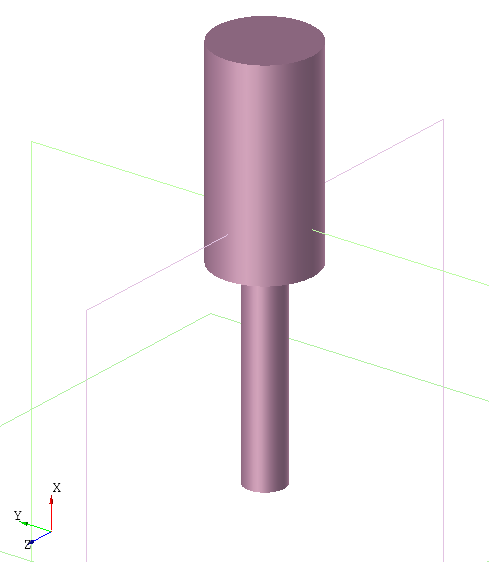
\includegraphics[width=0.45\linewidth]{figs/iscad/gmsh_example_iscad.png}
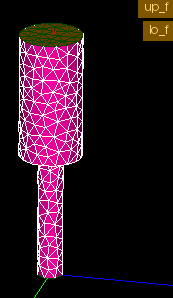
\includegraphics[width=0.45\linewidth]{figs/iscad/gmsh_example_mesh.png}
%![image](gmsh_example_iscad.png)
%![image](gmsh_example_mesh.png)

\subsection{Graphical Editor ISCAD}

ISCAD is a graphical editor for InsightCAD scripts. It
consists of a text editor for editing the script contents and a 3D view
and some other elements for inspecting the resulting model. A screenshot
is shown in the figure below.

The model script is entered into the text editor widget right of the 3D
display. Once a script shall be evaluated, it can be parsed by clicking
in the button "Rebuild" or pressing Ctrl+Return.

After parsing the model, the following results are displayed:

\begin{itemize}
\item A list of all created feature symbols in the "Model Steps" list box.
    If the check box is checked, the 3D geometry is displayed in the
    3D view.
\item The values of all scalars and vectors in the "Variables" list box.

    For each vector variable, a check box is displayed. If it is
    checked, the vector is interpreted as a point location and the point
    is shown in the 3D display window.

\item All defined datums are listed in the "Datums" list box. Again, the
    check box controls, whether the datum is displayed in the 3D view.
\end{itemize}
 

%![Screenshot of the ISCAD main window](screenshot_iscad.png)
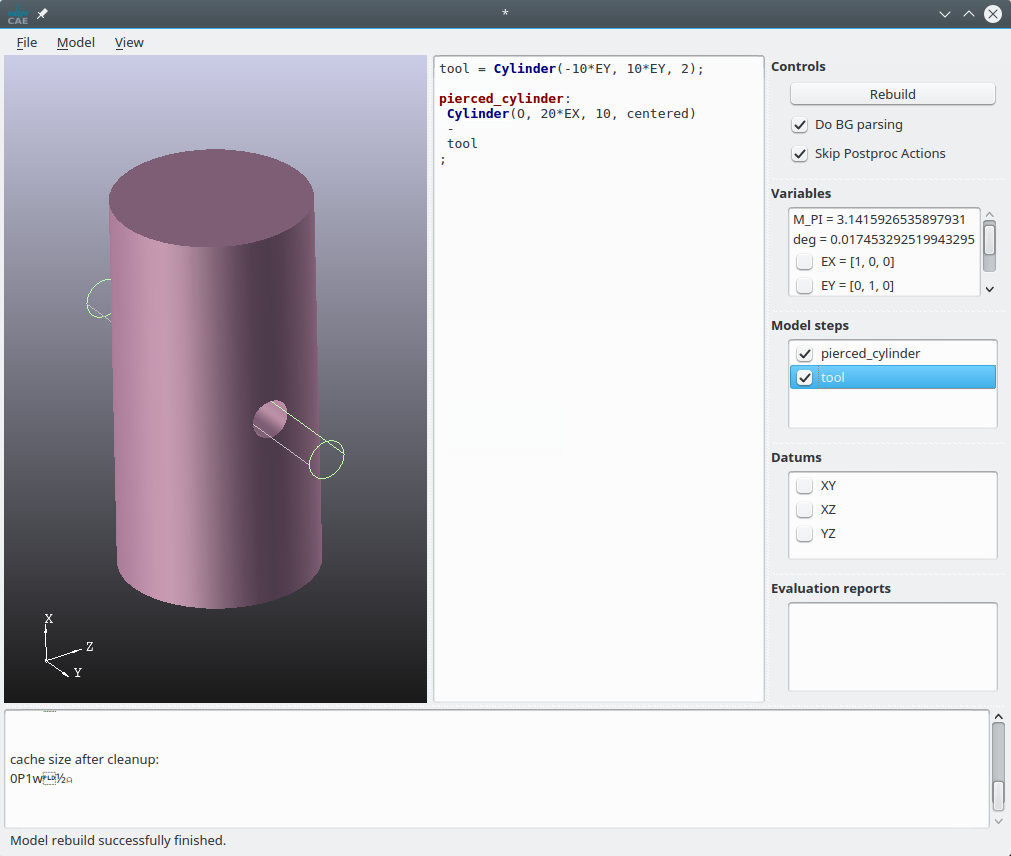
\includegraphics[width=\linewidth]{figs/iscad/screenshot_iscad}

\subsubsection{3D Graphics Display}

\paragraph{View Manipulation}

\begin{itemize}
\item Dragging: Shift + mouse move
\item Scaling: Ctrl + horizontal mouse move
\item Rotating: Alt + mouse move
\end{itemize}


\paragraph{Model Navigation}

When hoovering the mouse pointer over a displayed feature in the 3D
geometry window, it is highlighted. The highlighted feature is the one,
which would be selected during subsequent mouse clicks.

When the left mouse button is pressed, the highlighted feature is
selected and all its contained reference points are displayed.

When the right mouse button is pressed, a context menu for the selected
feature is displayed.

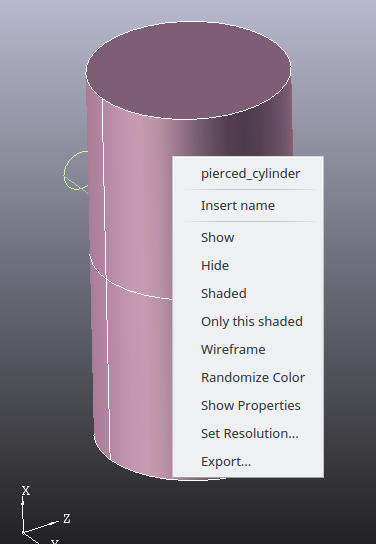
\includegraphics[width=0.33\linewidth]{figs/iscad/screen_iscad_contextmenu_3d}

The context menu provides these functions:

\begin{itemize}
\item The first entry is the feature name. When it is selected, the
    definition in the script editor is highlighted and the cursor jumps
    to it.
\item "Insert name": inserts the name of the feature symbol at the cursor
    location
\item "Export...": Export the feature geometry to a file (BREP, STP, IGES, STL)
\end{itemize}


\subsubsection{Text Editor}

When script code is entered into the text editor window, it is parsed in
the background. Once this has been done successfully, some extensions of
the context menu is available:

\begin{itemize}
\item Context menu on "Sketch" command:

    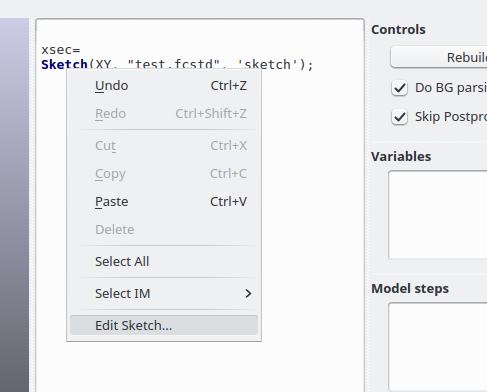
\includegraphics[width=0.33\linewidth]{figs/iscad/screenshot_iscad_context_sketch}
    
    When selecting the "Edit Sketch..." entry, FreeCAD is launched and
    the sketch editor opened. If the FreeCAD-file or sketch inside it is
    not yet existing, they are created.
\item Context menu on "loadmodel" command:

    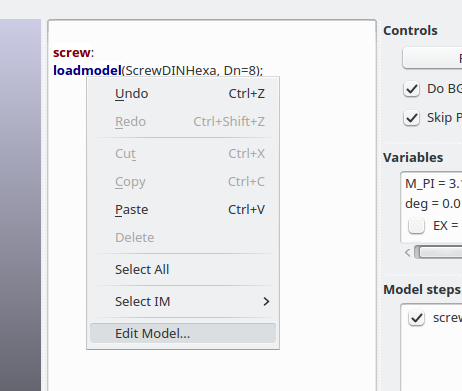
\includegraphics[width=0.33\linewidth]{figs/iscad/screenshot_iscad_context_loadmodel}
    
    When selecting the "Edit Model..." entry, another instance of iscad
    is launched with the specified model script loaded.
\end{itemize}
   
